\newpage
\section{The Other Side---Solving Equations}\label{A:otherSide}


In this activity, we will explore ideas related to solving equations.

\begin{prob}
Solve the following equation three ways: Using algebra, using the
balance, and with the graph. At each step, the three models should be in
complete alignment.
\[
\]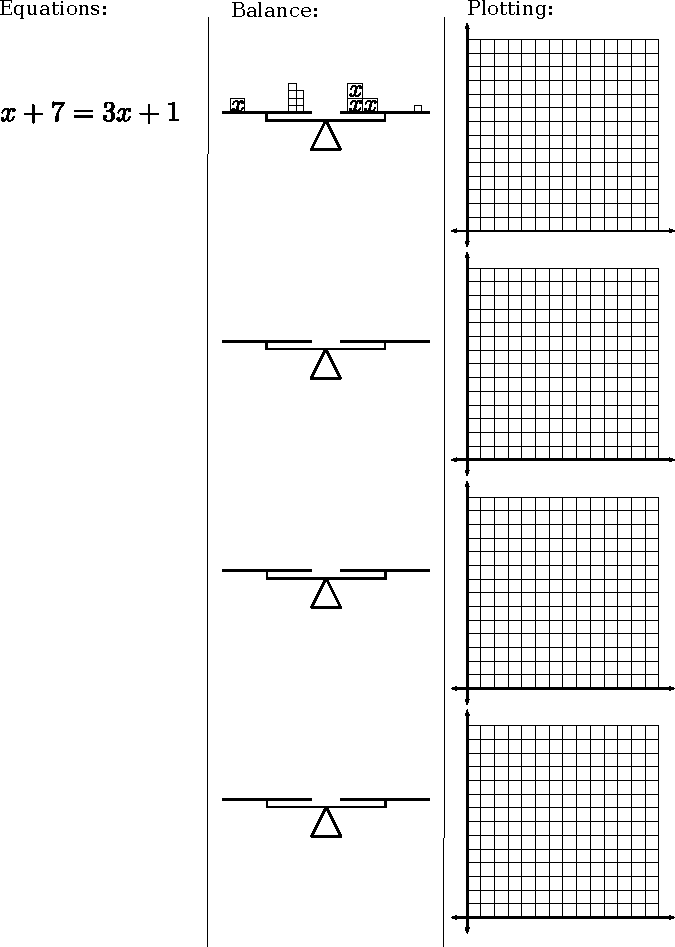
\includegraphics[scale=0.8]{../graphics/eqBalGraph.pdf}

\end{prob}

\begin{prob}
Critically analyze the three ``different'' methods of solving
equations. 
\end{prob}

\begin{prob}
Can you solve quadratic equations using the methods above?
If so give an example. If not, explain why not.
\end{prob}

\begin{teachingnote}
The key point here is that it is difficult to make ``balances'' work
for anything but linear equations.
\end{teachingnote}



\begin{prob}
Can you think of an example when the undoing via algebraic
manipulation would fail?
\end{prob}

\begin{teachingnote}
Here we are looking for something where an inverse function must be
applied, as in $.6 = \sin(x)$.
\end{teachingnote}


While sometimes we solve equations via a process of algebraic
manipulation, other times we have a formula.


\begin{prob}
Give a formula for solving linear equations of the form $ax + b =0$.
\end{prob}

\fixnote{Need a new activity for both completing the square and the zero-product property.}

%\begin{prob}
%Complete the square to give a formula for solving equations of the form
%\[
%x^2 + bx + c = 0.
%\]
%\end{prob}
%
%
%Of course these formulas can only take us so far. The key to solving
%polynomial equations is that finding any root will allow you to
%divide, and lower the degree.
%
%\begin{prob}
%Solve the following equation
%\[
%x^5 - 4x^4 - 18x^3 + 64x^2 + 17x -60 = 0
%\]
%assuming you know that $1$, $-1$, and $3$ are roots.
%\end{prob}


